\documentclass[10pt,letterpaper]{article}

\usepackage[margin=0.75in]{geometry}
\usepackage{tikz}

\begin{document}

  \title{CS 321, Assignment 6}
  \author{Cody Malick\\
  \texttt{malickc@oregonstate.edu}}
  \date{\today}
  \maketitle

\section{}
\subsection*{a}
Base case: Given some machine $M=\{Q,\Sigma,\delta,s,F\}$ and a CFG 
$G=\{A_p \rightarrow cA_q | \delta(p,c)\} 
\cup \{A_p \rightarrow \epsilon | p \in F\}$ with a start state $A_s = S$
where the start state has not read any characters. \\\\

$A_s = A_p \rightarrow cA_q$, where $|w|=1$\\\\

Inductive Step: We need to show that 


\subsection*{b}
Original: \\
\begin{center}
	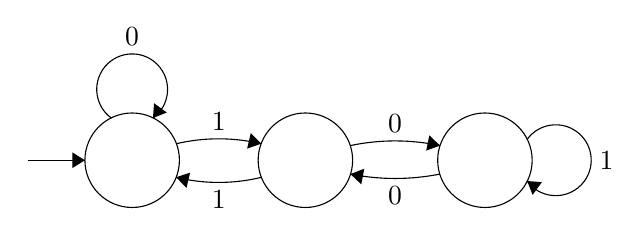
\begin{tikzpicture}[scale=0.2]
		\tikzstyle{every node}+=[inner sep=0pt]
		\draw [black] (12.4,-10.8) circle (3);
		\draw [black] (23.4,-10.8) circle (3);
		\draw [black] (34.8,-10.8) circle (3);
		\draw [black] (5.8,-10.8) -- (9.4,-10.8);
		\fill [black] (9.4,-10.8) -- (8.6,-10.3) -- (8.6,-11.3);
		\draw [black] (15.202,-9.752) arc (103.22544:76.77456:11.792);
		\fill [black] (20.6,-9.75) -- (19.93,-9.08) -- (19.7,-10.06);
		\draw (17.9,-8.94) node [above] {$1$};
		\draw [black] (26.246,-9.87) arc (101.89414:78.10586:13.848);
		\fill [black] (31.95,-9.87) -- (31.27,-9.22) -- (31.07,-10.19);
		\draw (29.1,-9.07) node [above] {$0$};
		\draw [black] (31.937,-11.68) arc (-78.79986:-101.20014:14.608);
		\fill [black] (26.26,-11.68) -- (26.95,-12.33) -- (27.14,-11.34);
		\draw (29.1,-12.46) node [below] {$0$};
		\draw [black] (20.612,-11.884) arc (-76.26827:-103.73173:11.425);
		\fill [black] (15.19,-11.88) -- (15.85,-12.56) -- (16.08,-11.59);
		\draw (17.9,-12.71) node [below] {$1$};
		\draw [black] (37.48,-9.477) arc (144:-144:2.25);
		\draw (42.05,-10.8) node [right] {$1$};
		\fill [black] (37.48,-12.12) -- (37.83,-13) -- (38.42,-12.19);
		\draw [black] (11.077,-8.12) arc (234:-54:2.25);
		\draw (12.4,-3.55) node [above] {$0$};
		\fill [black] (13.72,-8.12) -- (14.6,-7.77) -- (13.79,-7.18);
	\end{tikzpicture}
\end{center}

\noindent CFG:\\
$S \rightarrow 0S | 1T | \epsilon$\\
$T \rightarrow 1S | 0U$\\
$U \rightarrow 0T | 1U$\\

\section{}
Starting state:\\
$S \rightarrow aSddd\ |\ T$\\
$T \rightarrow bTdd\ |\ R$\\
$R \rightarrow cR\ |\ \epsilon$\\

Step 1, add new start symbol $S^*$, add rule $S^* \rightarrow S$\\
$S^* \rightarrow S$\\
$S \rightarrow aSddd\ |\ T$\\
$T \rightarrow bTdd\ |\ R$\\
$R \rightarrow cR\ |\ \epsilon$\\

Step 2, Shorten RHS rules for each rule $A \rightarrow \alpha_1, \alpha_2,...,\alpha_k$
where $k \geq 3$\\
$S^* \rightarrow S$\\
$S \rightarrow MN\ |\ T$\\
$M \rightarrow aS$\\
$N \rightarrow dO$\\
$O \rightarrow dd$\\
$T \rightarrow PO\ |\ R$\\
$P \rightarrow bT$\\
$R \rightarrow cR\ |\ \epsilon$\\

Step 3, Clean up mixed RHS\\
$S^* \rightarrow S$\\
$S \rightarrow MN\ |\ T$\\
$M \rightarrow AS$\\
$N \rightarrow DO$\\
$O \rightarrow DD$\\
$T \rightarrow PO\ |\ R$\\
$P \rightarrow BT$\\
$R \rightarrow CR\ |\ \epsilon$\\
$A \rightarrow a$\\
$B \rightarrow b$\\
$C \rightarrow c$\\

Step 4, determine which nonterminal are "nullable" $(A \Rightarrow^* \epsilon)$\\
The only rule that goes to $\epsilon$ is R, so:\\
$S^* \rightarrow S$\\
$S \rightarrow MN\ |\ T$\\
$M \rightarrow AS$\\
$N \rightarrow DO$\\
$O \rightarrow DD$\\
$T \rightarrow PO\ |\ C$\\
$P \rightarrow BT$\\
$A \rightarrow a$\\
$B \rightarrow b$\\
$C \rightarrow c$\\

Step 5, for each rule $A \rightarrow B$, copy all $B \rightarrow \alpha$ rules to
$A \rightarrow \alpha$. Repeat until no more changes, then delete $A \rightarrow B$\\
$S^* \rightarrow MN\ |\ TS$\\
$M \rightarrow AS$\\
$N \rightarrow DO$\\
$O \rightarrow DD$\\
$T \rightarrow PO\ |\ c$\\
$P \rightarrow BT$\\
$A \rightarrow a$\\
$B \rightarrow b$\\
$C \rightarrow c$\\



\section{}
\subsection*{a}
\subsection*{b}
\end{document}
